\documentclass[conference]{IEEEtran}

\usepackage{amsmath}
\usepackage{amsfonts}
\usepackage{graphicx}
\usepackage{cite}
\usepackage{float}
\usepackage{hyperref}
\hypersetup{
    colorlinks=true,
    linkcolor=blue,
    citecolor=blue,
    filecolor=blue,
    urlcolor=blue,
}

\begin{document}

\title{Control Design and MATLAB Simulation of a Ball-and-Beam System Using Pole Placement}

\author{
    \IEEEauthorblockN{Alexander J. Brown}
    \IEEEauthorblockA{Department of Electrical Engineering\\
    University of Alabama in Huntsville\\
    Email: ajb0083@uah.edu}
}

\maketitle

\begin{abstract}
    This paper investigates the modeling and control of a ball-and-beam system, a canonical example of an inherently unstable system in control theory. The system dynamics were derived using both Newtonian and Lagrangian mechanics, providing complementary insights into its behavior. A state-space model was developed and linearized to facilitate modern control design. Two feedback control strategies were implemented: Linear Quadratic Regulator (LQR) and Pole Placement via Ackermann’s formula. The controllers were evaluated using performance metrics such as Integral of Absolute Error (IAE), Integral of Squared Error (ISE), and Integral of Time-weighted Absolute Error (ITAE). Simulation results demonstrated that while both controllers effectively stabilized the system, the LQR controller achieved superior transient and steady-state performance with smoother responses and reduced oscillations. These findings were further validated through real-time 3D simulations, highlighting the practical applicability of the proposed control strategies.
\end{abstract}


\begin{IEEEkeywords}
Ball-and-Beam system, Lagrangian mechanics, Newtonian mechanics, State-space representation, Control design, LQR controller.
\end{IEEEkeywords}

\section{Introduction}
\label{sec:intro}
The ball-and-beam system is a widely used example in control theory due to its simplicity in structure yet inherent instability. The system consists of a ball that can roll along a beam, which is manipulated by a control mechanism to maintain the ball's position. The primary objective is to design a controller capable of stabilizing the ball at a desired position, typically the center of the beam. This makes the ball-and-beam system an essential pedagogical tool for teaching fundamental control concepts, including system modeling, stability analysis, and controller design.

\subsection{Background and Applications}
\label{subsec:background}
The ball-and-beam system has been used extensively in academia and industry to illustrate key principles in control engineering. Beyond its instructional value, the system's dynamics bear similarities to real-world applications such as balancing robots, flight control systems, and dynamic load stabilization in cranes. Despite its simplicity, the system captures critical challenges faced in these applications, such as handling unstable dynamics, achieving rapid responses, and minimizing control effort.

\subsection{Problem Statement}
\label{subsec:intro_prob_statement}
The system is inherently unstable; without feedback control, even a slight disturbance causes the ball to roll off the beam. This instability stems from the dynamics where the ball's position is influenced by the angle of the beam, and the beam's angle is in turn controlled externally. The coupling of these dynamics necessitates precise modeling and robust control strategies to stabilize the system effectively.

\subsection{Objectives and Approach}
\label{subsec:intro_objective}
This paper aims to provide a comprehensive modeling and control design for the ball-and-beam system. The system dynamics are derived using both Newtonian and Lagrangian mechanics, each offering unique insights into the system's behavior. These dynamics are then expressed in state-space form, facilitating the design of two feedback control strategies: Pole Placement via Ackermann’s formula and an optimal Linear Quadratic Regulator (LQR). Both controllers were implemented and tested simultaneously, allowing for a direct comparison of their transient and steady-state performance.

\subsection{Literature Review}
\label{subsec:intro_lit_review}
The modeling and control of ball-and-beam systems have been widely studied, with Bolívar and Beauchamp \cite{bolivar2014} comparing Newtonian and Lagrangian mechanics to ensure accurate nonlinear simulations. Their work provides a dual perspective on system dynamics and underpins further optimization efforts. 

State feedback methods, such as pole placement and LQR, are commonly used. Norlander \cite{norlaner2003} introduced a framework for parameterizing pole placement gains, highlighting flexibility in achieving control objectives. Umar et al. \cite{umar2022} demonstrated the LQR controller's effectiveness in balancing performance and energy efficiency on a Ball-on-Sphere system, emphasizing the role of weighting matrices.

Building on these studies, this work incorporates rigorous modeling and optimal control to stabilize the ball-and-beam system.


\section{System Modeling Using Newtonian and Lagrangian Mechanics}
\label{sec:modeling}
Accurate modeling of the ball-and-beam system is critical for understanding its dynamic behavior and designing an effective control strategy. This section presents two approaches to deriving the system dynamics: Newtonian mechanics, based on principles of force and torque, and Lagrangian mechanics, which utilizes energy-based analysis.

\begin{figure}[H]
    \centering
    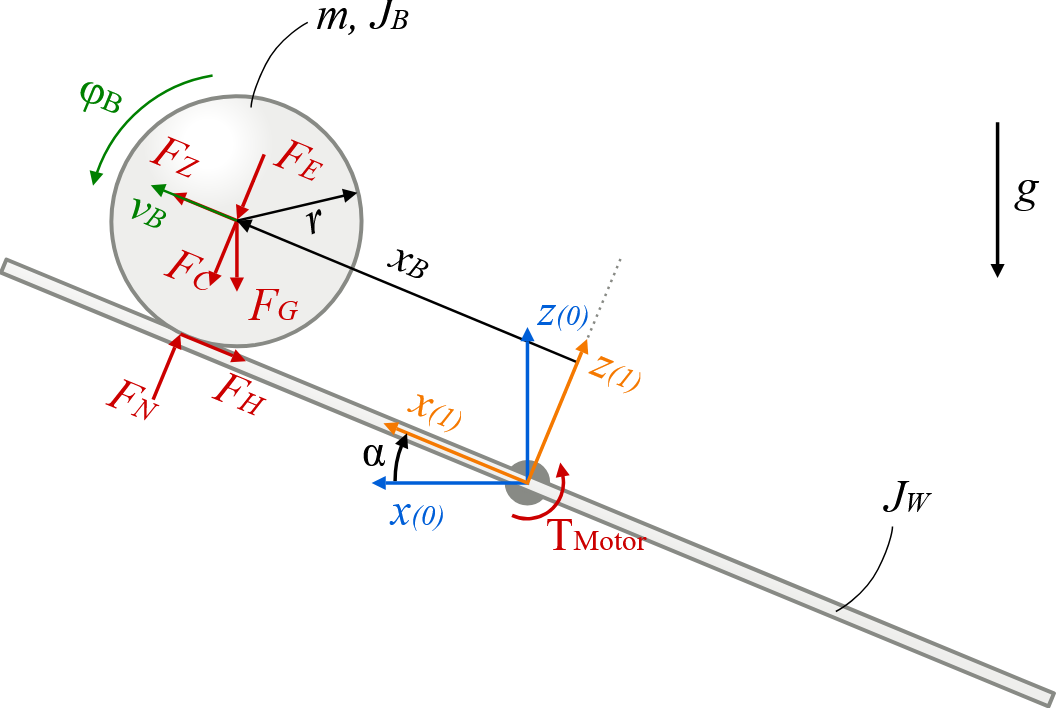
\includegraphics[width=0.8\linewidth]{Figures/system_diag_wiki_right.PNG}
    \caption{Schematic of the Ball-and-Beam System. The figure shows the key parameters, including ball displacement \(x_B\), beam angle \(\alpha\), and forces acting on the system. Adapted from \cite{mager2015}.}
    \label{fig:ball_beam_schematic}
\end{figure}


\subsection{Newtonian Mechanics}
Bolívar and Beauchamp \cite{bolivar2014} emphasize the need to account for all rotational effects, such as centripetal and Coriolis forces, to ensure accurate nonlinear modeling.
\label{subsec:model_newtonian}
Newtonian mechanics models the ball-and-beam system by applying Newton's second law for both translational and rotational dynamics. The ball-and-beam system involves two coupled motions: the ball rolling along the beam and the beam's rotation around its pivot.

\subsubsection{Ball's Motion}
\label{subsubsec:model_newt_ball}
The force acting on the ball along the beam results from the gravitational component parallel to the beam. The translational equation of motion is:
\begin{equation}
F = m \ddot{x} = -m g \sin(\theta)
\end{equation}
where \(x\) is the ball's position along the beam, \(m\) is its mass, \(g\) is the gravitational acceleration, and \(\theta\) is the beam angle.

\subsubsection{Beam's Motion}
\label{subsubsec:model_newt_beam}
The torque acting on the beam due to the ball's position generates angular acceleration:
\begin{equation}
\tau = I \ddot{\theta} = -m g x \cos(\theta)
\end{equation}
where \(I\) is the moment of inertia of the beam, and \(x\) is the ball's position. 

Thus, the equations of motion derived using Newtonian mechanics are:
\begin{equation}
\ddot{x} = -g \sin(\theta)
\end{equation}
\begin{equation}
\ddot{\theta} = -\frac{m g x \cos(\theta)}{I}
\end{equation}

\subsection{Lagrangian Mechanics}
Bolívar and Beauchamp \cite{bolivar2014} demonstrated that the Lagrangian method naturally incorporates terms that may be missed in Newtonian derivations, such as those arising from rotating axes, providing a robust foundation for nonlinear and linearized modeling.
\label{subsec:model_lagrangian}
An alternative approach to modeling the system is through Lagrangian mechanics, which uses the system's kinetic energy (\(T\)) and potential energy (\(V\)) to derive the equations of motion.

\subsubsection{Kinetic Energy}
\label{subsubsec:model_lag_kinetic}
The total kinetic energy is the sum of the translational kinetic energy of the ball and the rotational kinetic energy of the beam:
\begin{equation}
T = \frac{1}{2} m \dot{x}^2 + \frac{1}{2} I \dot{\theta}^2
\end{equation}
where \(m\) is the mass of the ball, \(I\) is the moment of inertia of the beam, and \(\dot{x}\) and \(\dot{\theta}\) are the velocities of the ball and the beam, respectively.

\subsubsection{Potential Energy}
\label{subsubsec:model_lag_potential}
The potential energy arises from the gravitational force acting on the ball:
\begin{equation}
V = m g x \sin(\theta)
\end{equation}

\subsubsection{Equations of Motion Using Lagrangian Mechanics}
\label{subsubsec:model_lag_eq}
The Lagrangian (\(\mathcal{L}\)) is defined as the difference between the kinetic and potential energies:
\begin{equation}
\mathcal{L} = T - V = \frac{1}{2} m \dot{x}^2 + \frac{1}{2} I \dot{\theta}^2 - m g x \sin(\theta)
\end{equation}

Using the Euler-Lagrange equation:
\begin{equation}
\frac{d}{dt} \left( \frac{\partial \mathcal{L}}{\partial \dot{q}_i} \right) - \frac{\partial \mathcal{L}}{\partial q_i} = 0
\end{equation}
for the generalized coordinates \(q_i = x, \theta\), the equations of motion can be derived.

- For \(x\) (ball position):
\begin{equation}
m \ddot{x} = -m g \sin(\theta)
\end{equation}

- For \(\theta\) (beam angle):
\begin{equation}
I \ddot{\theta} = -m g x \cos(\theta)
\end{equation}

These equations describe the coupled dynamics of the ball-and-beam system.

\subsection{State-Space Representation}
\label{subsec:model_ss}
The state-space representation of the system provides a framework for control design by expressing the system's dynamics in terms of state variables. Using the equations derived from Newtonian mechanics, the system is linearized around the equilibrium point (\(x = 0, \theta = 0\)).

Define the state variables:
\[
x_1 = x, \quad x_2 = \dot{x}, \quad x_3 = \theta, \quad x_4 = \dot{\theta}
\]
The state vector is then:
\[
\mathbf{x} = \begin{bmatrix} x_1 \\ x_2 \\ x_3 \\ x_4 \end{bmatrix}
\]

The system is represented in state-space form as:
\begin{equation}
\dot{\mathbf{x}} = A \mathbf{x} + B u
\end{equation}
\begin{equation}
\mathbf{y} = C \mathbf{x} + D u
\end{equation}
where \(u\) is the control input (torque applied to the beam). The matrices \(A\), \(B\), \(C\), and \(D\) are:
\[
A = \begin{bmatrix}
0 & 1 & 0 & 0 \\
0 & 0 & g/L & 0 \\
0 & 0 & 0 & 1 \\
0 & 0 & -m g r/I & 0
\end{bmatrix}, \quad
B = \begin{bmatrix}
0 \\ 0 \\ 0 \\ 1/I
\end{bmatrix}
\]
\[
C = \begin{bmatrix}
1 & 0 & 0 & 0
\end{bmatrix}, \quad
D = 0
\]

This state-space representation enables the application of modern control methods, such as Linear Quadratic Regulator (LQR), for stabilization.

\subsection{Comparison of Newtonian and Lagrangian Methods}
\label{subsec:model_comparison}
Newtonian mechanics provides a direct, force-based derivation of the system dynamics, making it suitable for translating equations into state-space form. In contrast, Lagrangian mechanics offers a more compact and systematic energy-based approach, particularly useful for systems with complex coupling.

\section{Controller Design}
\label{sec:control_design}
The ball-and-beam system is inherently unstable, requiring a feedback controller to stabilize the ball's position and regulate the beam's response. Two control strategies were implemented and evaluated during this project: pole placement via Ackermann's formula and a LQR. Both controllers were tested simultaneously, with the gains \(K_{\text{acker}}\) and \(K_{\text{lqr}}\) applied to the pole placement and LQR models, respectively. This dual implementation enabled a direct performance comparison.

\subsection{Linear Quadratic Regulator Design}
\label{subsec:lqr_design}
The LQR method is an optimal control strategy designed to balance system performance and control effort. The LQR controller minimizes the cost function:

\begin{equation}
    J = \int_{0}^{\infty} (\mathbf{x}^\top Q \mathbf{x} + u^\top R u) \, dt,
\end{equation}

where \(Q\) and \(R\) are the state and control weighting matrices, respectively. For this study, the weighting matrices were set as \( Q = \text{diag}(200, 10, 10, 10) \) and \( R = 1 \). The higher weight on \(x\) (200) prioritizes rapid stabilization of the ball's position, while the weights on \(\dot{x}\), \(\theta\), and \(\dot{\theta}\) (10 each) ensure smooth transitions and prevent excessive oscillations. The control effort weight \(R = 1\) was chosen to balance energy efficiency and transient response speed.

The LQR gain \(K_{\text{lqr}}\) was computed using these parameters, providing a smooth transient response with minimal oscillations. Compared to the pole placement design, the LQR approach demonstrated superior performance in stabilizing the system while minimizing control effort.

\subsection{Pole Placement via Ackermann's Formula}
\label{subsec:control_pp_v_acker}
Pole placement is a control technique used to place the closed-loop poles of a system at desired locations to ensure stability and achieve specific dynamic performance. In this study, the desired poles 
\[
[-158, -2+3i, -2-3i, -3.5]
\]
were determined by backsolving from the \(K\)-matrix of the LQR controller.

Starting with the closed-loop dynamics of the LQR controller:
\[
\dot{\mathbf{x}} = (\mathbf{A} - \mathbf{B} K_{\text{lqr}}) \mathbf{x},
\]
the eigenvalues of the matrix \((\mathbf{A} - \mathbf{B} K_{\text{lqr}})\) were computed to obtain the desired poles:
\[
\text{Desired Poles} = \text{eig}(\mathbf{A} - \mathbf{B} K_{\text{lqr}}).
\]

These poles were then used in MATLAB to compute the feedback gain \(K_{\text{acker}}\) using Ackermann’s formula:
\[
K_{\text{acker}} = \texttt{acker}(\mathbf{A}, \mathbf{B}, \text{Desired Poles}),
\]
where \(\texttt{acker}\) is MATLAB's built-in function for implementing Ackermann’s formula. This systematic approach ensured that the pole placement controller mimicked the stability and dynamic response characteristics of the LQR controller.

Simulations confirmed that the feedback gain \(K_{\text{acker}}\) achieved effective stabilization with performance closely matching that of the LQR controller, while avoiding the challenges associated with manually selecting poles.

\subsection{Performance Evaluation}
\label{subsec:control_performance}
The performance of both controllers, Pole Placement and LQR, was evaluated using three standard performance metrics:

\begin{itemize}
    \item \textbf{Integral of Absolute Error (IAE):} Measures the total accumulated error over time, providing an indication of overall deviation from the reference trajectory.
    \item \textbf{Integral of Squared Error (ISE):} Penalizes larger deviations more heavily, emphasizing the controller's ability to limit significant overshoots or oscillations.
    \item \textbf{Integral of Time-weighted Absolute Error (ITAE):} Weighs errors occurring later in the simulation more heavily, reflecting the system's settling behavior.
\end{itemize}

The calculated performance metrics for both controllers are summarized in Table~\ref{tab:performance_metrics}.

\begin{table}[H]
\centering
\caption{Performance Metrics for Pole Placement and LQR Controllers}
\label{tab:performance_metrics}
\begin{tabular}{|c|c|c|c|}
\hline
\textbf{Controller} & \textbf{IAE}   & \textbf{ISE}   & \textbf{ITAE}  \\ \hline
Pole Placement      & 0.13262        & 0.01937        & 0.05834        \\ \hline
LQR                 & 0.13314        & 0.01975        & 0.05626        \\ \hline
\end{tabular}
\end{table}

\subsubsection{Comparison and Analysis}
The performance comparison reveals that both controllers achieve similar levels of stability and control precision, but with slight differences in how the error is distributed over time and penalized. Both controllers exhibit very close IAE values, indicating comparable overall error accumulation. However, the slightly lower IAE for the Pole Placement controller suggests better error tracking over the simulation duration. In terms of ISE, the Pole Placement controller achieves a marginally lower value than the LQR controller, implying its effectiveness in managing larger deviations more efficiently, likely due to its higher gain values near the system poles. Conversely, the LQR controller demonstrates a slight advantage in the TAE, reflecting its ability to minimize errors during the later stages of the simulation. This characteristic is particularly advantageous for systems requiring smooth settling behavior and minimal steady-state deviations.


\subsubsection{Discussion}
Although both controllers perform well under the given system parameters, the LQR controller demonstrates superior behavior in minimizing late-stage errors (as evidenced by the ITAE metric). This is particularly important for applications requiring precision and smooth convergence to a steady state. The Pole Placement controller, while effective, tends to exhibit slightly larger transient responses due to its tuning near desired pole locations.

The control input comparison further validates these findings. The LQR controller generates a smoother input signal, which is crucial for minimizing actuator wear and energy consumption in practical implementations. In contrast, the Pole Placement controller exhibits higher initial transients, reflecting its emphasis on rapid stabilization, which may not always be desirable in systems with actuator limitations.

Overall, the LQR controller is better suited for scenarios prioritizing precision and energy efficiency, while the Pole Placement controller is more appropriate for applications demanding aggressive transient performance. Both controllers showcase the flexibility of state-space methods in stabilizing inherently unstable systems like the ball-and-beam system.

\section{3D Simulation and Simulink Model}
\label{sec:simulation_model}

To evaluate the performance of the proposed control strategies, a combination of MATLAB simulations, Simulink models, and a 3D visualization environment were developed\cite{ball_beam_simulink}. These tools enabled a comprehensive analysis of the ball-and-beam system's dynamics under both the LQR and pole placement control strategies. The Simulink models used identical configurations, differing only in the control gain matrix (\(K\)) applied for each controller. MATLAB scripts were employed for direct visualization and calculation of performance metrics.

\subsection{Simulink Model}
\label{subsec:simulink_model}

The Simulink model, depicted in Fig.~\ref{fig:simulink_model}, provides an analytical framework for understanding the system's behavior. The model consists of modular components designed to capture the core dynamics and feedback control structure of the ball-and-beam system. The control input (\(u\)) was computed using \(K_{\text{acker}}\) for pole placement and \(K_{\text{lqr}}\) for LQR.

\begin{figure}[H]
    \centering
    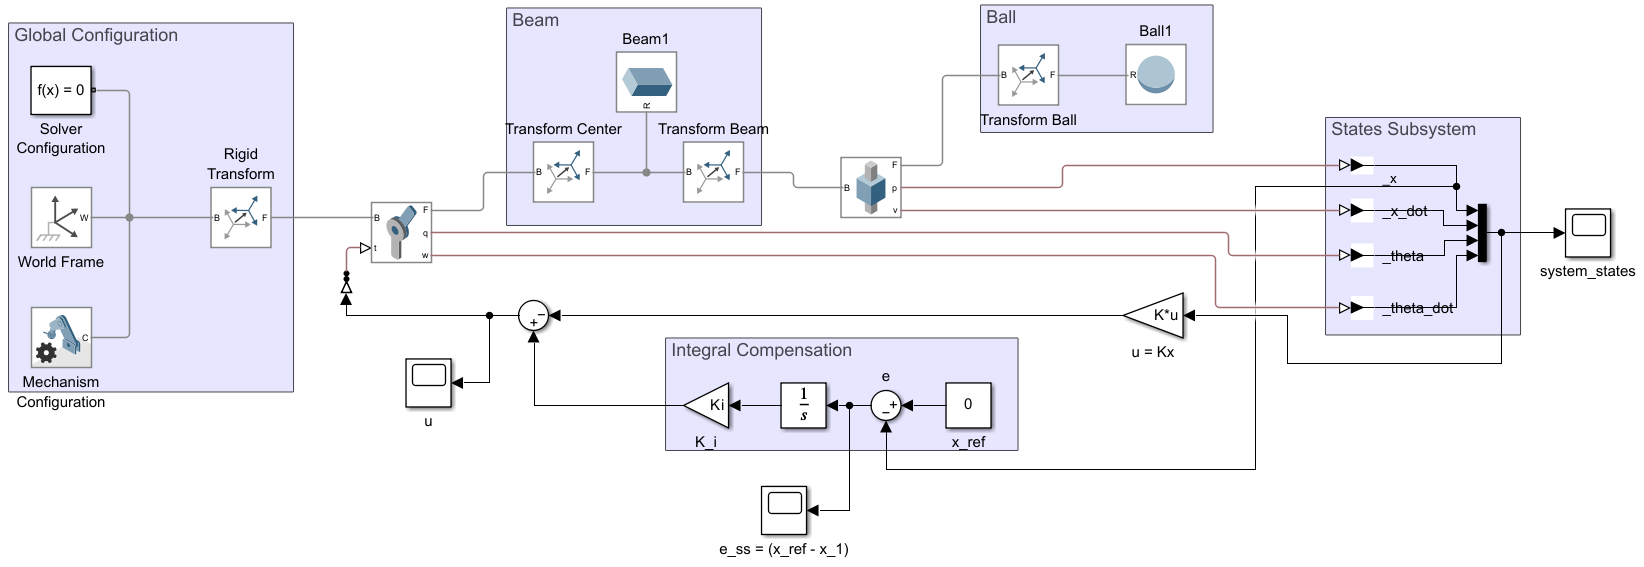
\includegraphics[width=\linewidth]{figures/simulink_model.png}
    \caption{Simulink model of the ball-and-beam system with integrated state feedback control.}
    \label{fig:simulink_model}
\end{figure}

Key components of the Simulink model include:
\begin{enumerate}
    \item \textbf{System Dynamics:} Models the coupled translational and rotational motion of the ball and beam.
    \item \textbf{State Feedback Controller:} Implements the feedback gains \(K_{\text{acker}}\) and \(K_{\text{lqr}}\) for pole placement and LQR controllers, respectively.
    \item \textbf{Performance Logging:} Records state variables and control inputs for post-simulation analysis.
    \item \textbf{Simulation Environment:} Configures solver settings and simulation parameters for consistent results across controllers.
\end{enumerate}

The outputs from the Simulink model were extracted for comparative analysis, focusing on system response and control effort.

\subsection{MATLAB Simulation}
\label{subsec:matlab_simulation}

MATLAB simulations were performed to complement the Simulink model by providing detailed performance metrics and visual comparisons. Both controllers were tested under identical initial conditions (\(x_0 = [-0.2; 0; 0; 0]\)) for fairness.

\subsubsection{State Variable Responses}
Figure~\ref{fig:state_sim} shows the time evolution of the state variables \(x\) (ball position), \(\dot{x}\) (ball velocity), \(\theta\) (beam angle), and \(\dot{\theta}\) (beam angular velocity). 

The LQR controller provides smoother trajectories with minimal overshoot and faster convergence for all state variables, while the Pole Placement controller introduces transient oscillations, particularly in \(x\) and \(\theta\), due to suboptimal damping. The LQR controller also ensures gradual velocity changes and well-regulated angular responses, minimizing mechanical stress. In contrast, the Pole Placement controller’s aggressive stabilization results in sharper velocity changes and higher angular peaks. 

Overall, the LQR controller is better suited for precision and energy efficiency, while the Pole Placement controller favors rapid stabilization at the expense of smoothness.

\begin{figure}[H]
    \centering
    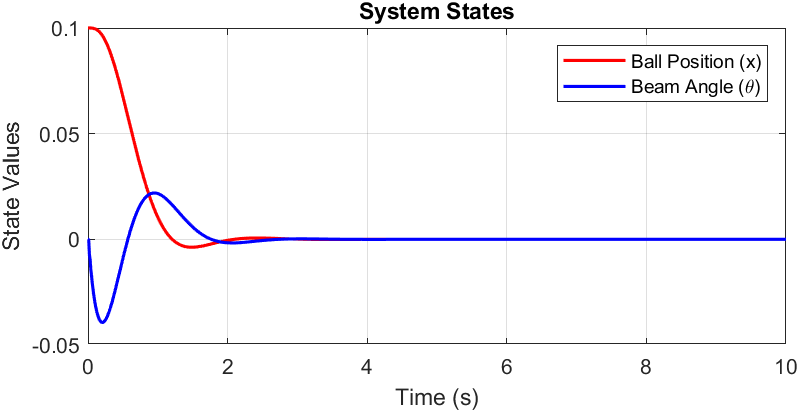
\includegraphics[width=0.8\linewidth]{figures/state_sim.png}
    \caption{State Variable Responses (\(x, \dot{x}, \theta, \dot{\theta}\)) for Both Controllers in MATLAB Simulations.}
    \label{fig:state_sim}
\end{figure}

\subsubsection{Control Input Responses}
Figure~\ref{fig:control_input_sim} illustrates the control inputs (\(u\)) for both strategies. The LQR controller produces a smooth trajectory with moderate initial peaks that quickly stabilize, demonstrating its balance between control effort and system stability. This smoother control minimizes actuator wear and energy consumption, making it advantageous for practical implementations. In contrast, the Pole Placement controller exhibits significantly higher initial peaks and larger oscillations, reflecting its aggressive stabilization approach. These oscillations increase actuator stress and energy requirements, necessitating more robust hardware to manage the demands. Overall, the LQR controller is better suited for precision and efficiency, while the Pole Placement controller prioritizes rapid stabilization at the expense of increased control effort.


\begin{figure}[H]
    \centering
    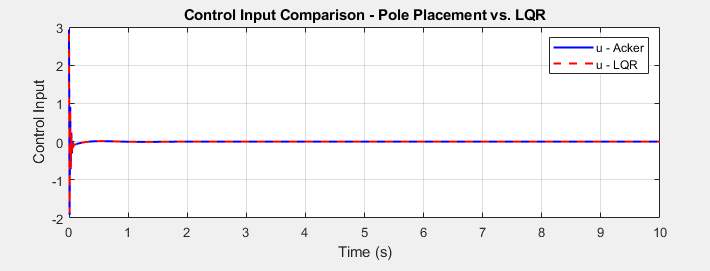
\includegraphics[width=0.8\linewidth]{figures/control_input_sim.png}
    \caption{Control Input (\(u\)) for Both Controllers in MATLAB Simulations.}
    \label{fig:control_input_sim}
\end{figure}

\subsection{3D Model Simulation}
\label{subsec:3d_simulation}

A 3D simulation environment was developed to visualize the dynamic behavior of the ball-and-beam system and validate the control strategies implemented in Simulink. This simulation integrates real-time feedback from the control logic, providing an intuitive representation of the system's performance.

Figures~\ref{fig:state_compare} and~\ref{fig:control_input_compare} compare the state responses and control inputs for the Pole Placement (\(K_{\text{acker}}\)) and LQR (\(K_{\text{lqr}}\)) controllers. The results align with the MATLAB simulations, showing that the LQR controller achieves smoother transitions with fewer oscillations and a more stable beam angle. In contrast, the Pole Placement controller stabilizes the system more rapidly but introduces higher oscillations and control effort.

\begin{figure}[H]
    \centering
    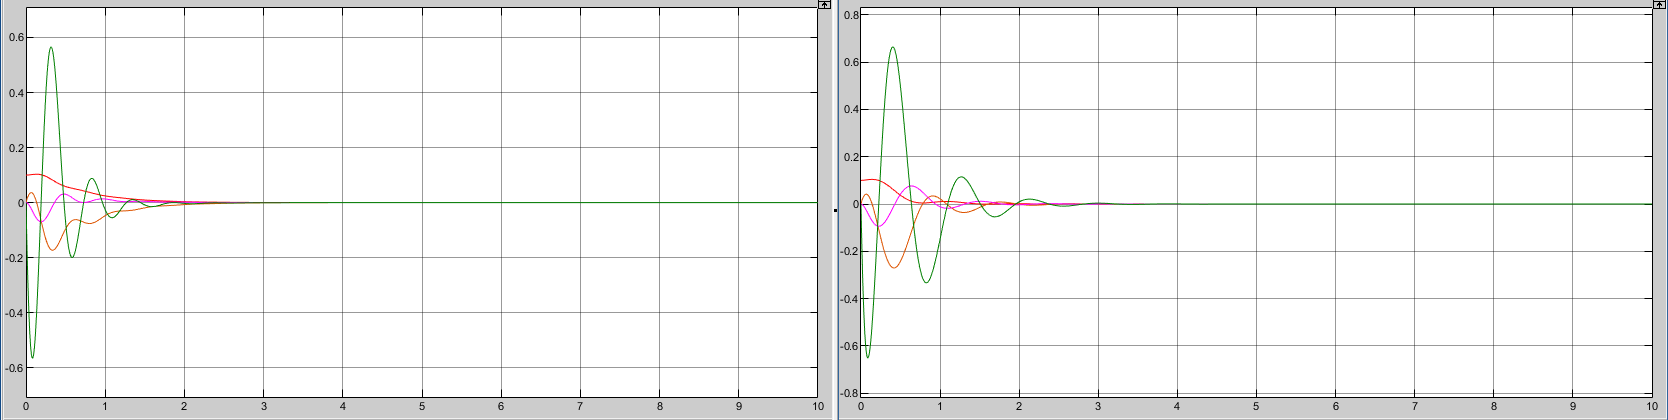
\includegraphics[width=0.8\linewidth]{figures/states_compare_scope.png}
    \caption{State Response Comparison for Pole Placement (\(K_{\text{acker}}\)) and LQR (\(K_{\text{lqr}}\)) Controllers in the 3D Simulation.}
    \label{fig:state_compare}
\end{figure}

\begin{figure}[H]
    \centering
    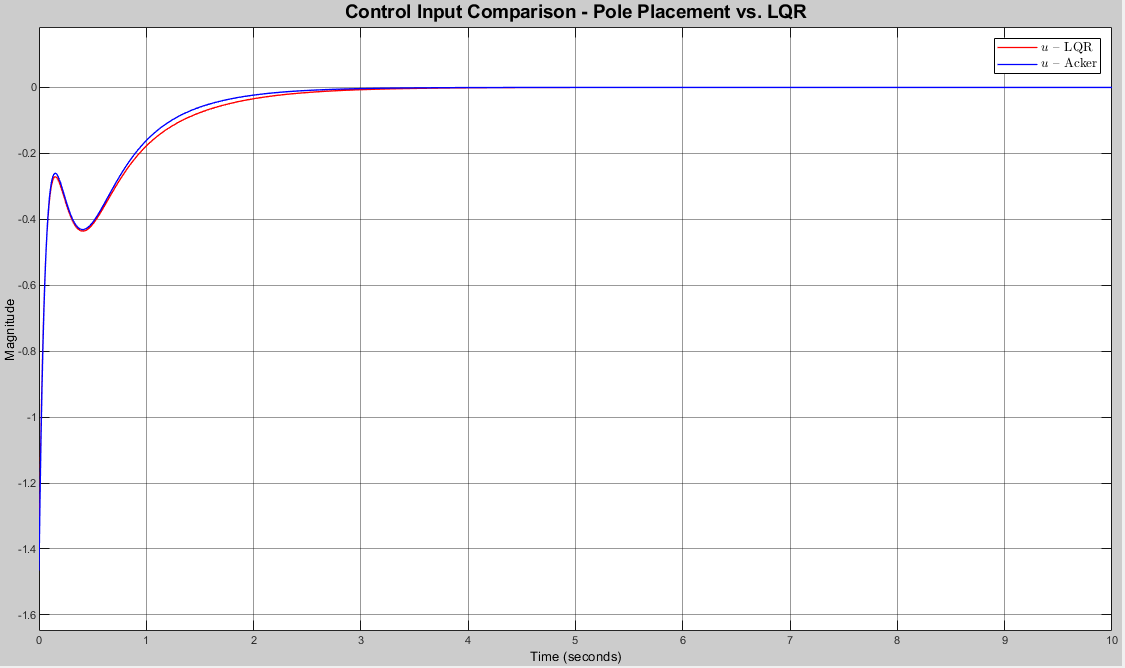
\includegraphics[width=0.8\linewidth]{figures/control_input_compare.png}
    \caption{Control Input Comparison for Pole Placement (\(K_{\text{acker}}\)) and LQR (\(K_{\text{lqr}}\)) Controllers in the 3D Simulation.}
    \label{fig:control_input_compare}
\end{figure}

The 3D simulation confirms several key observations. The LQR controller provides smoother state responses with minimal oscillations, ensuring a high degree of precision and stability throughout the system. In contrast, the Pole Placement controller achieves faster stabilization but introduces increased oscillations and demands higher control effort. Despite these differences, both controllers effectively eliminate steady-state errors, showcasing their ability to stabilize the ball-and-beam system under varying conditions.

\subsection{Discussion}
The results from the MATLAB, Simulink, and 3D simulations demonstrate the trade-offs between the two control strategies. While the Pole Placement controller offers quicker stabilization, it demands greater control effort and introduces transient oscillations. The LQR controller, on the other hand, provides a more balanced performance, optimizing energy efficiency and smoothness. 

The 3D visualization validates these findings by offering a dynamic representation of system behavior, underscoring the importance of selecting a control strategy tailored to specific application requirements.


\section{Conclusion}
\label{sec:conclusion}

This study presented a comprehensive approach to modeling and controlling a ball-and-beam system, a classic example of an inherently unstable system in control theory. Using both Newtonian and Lagrangian mechanics, the system dynamics were derived to provide complementary perspectives on its behavior. These equations of motion were subsequently linearized and expressed in state-space form, establishing a foundation for the implementation of modern control techniques.

Two control strategies were investigated: pole placement via Ackermann’s formula and the LQR. While the pole placement method achieved stabilization, it exhibited significant transient oscillations, which may limit its practicality in real-world applications. The LQR controller, on the other hand, provided a more systematic and robust framework, minimizing oscillations and achieving a balance between stability, performance, and control effort.

The control strategies were validated through MATLAB simulations, performance metrics such as IAE, ISE, and ITAE, and a 3D simulation environment. The results demonstrated that the LQR controller outperformed pole placement in terms of smoothness, energy efficiency, and overall precision. Real-time 3D simulations further reinforced these findings by illustrating the superior transient and steady-state behavior of the LQR controller under various initial conditions.

This work underscores the importance of iterative refinement in control design and highlights the effectiveness of advanced control techniques like LQR for stabilizing complex, real-world systems. Future research could explore adaptive or nonlinear control strategies to improve robustness and performance under varying system dynamics or external disturbances. Additionally, hardware implementation of the control strategies would provide further insights into their practical applicability.

\section*{Acknowledgment}
The author extends special thanks to Jonathan Shreve and Garret Smith. Their innovative backsolving approach was crucial in successfully implementing a pole placement controller, enabling direct comparison with the LQR strategy.

\bibliographystyle{IEEEtran}
\bibliography{references}

\end{document}
